\chapter{OBDD e Model Checking Simbolico}\label{ch:obdd}

Gli algoritmi di model checking visti finora lavorano \emph{esplicitamente} sugli stati del modello: etichettano stati, visitano archi, calcolano preimmagini enumerando predecessori. Il problema è che lo spazio degli stati dei sistemi reali cresce esponenzialmente con il numero di componenti e variabili (\keyword{state explosion}): serve un modo per rappresentare e manipolare insiemi di stati \emph{in modo simbolico}, ovvero tramite le loro funzioni caratteristiche, senza mai enumerarli.

In questo capitolo introduciamo i \keyword{Binary Decision Diagram} (BDD) e la loro versione ordinata (OBDD), una struttura dati per rappresentare funzioni booleane in modo canonico e compatto, e mostriamo come implementare su di essi l'algoritmo di model checking di CTL a punto fisso del capitolo precedente.

\section{Dalle tabelle di verità ai BDD}

Per rappresentare efficientemente le funzioni booleane passeremo per gli alberi di decisione, da cui poi, eliminando la ridondanza, arriveremo ai BDD, che sono DAG\@.

\subsection{La forma normale if-then-else}

Questa rappresentazione è fortemente legata alla forma normale \keyword{ITE} (if-then-else). Introduciamo un operatore booleano ternario \(\phi \to \phi_1,\phi_2\), che intuitivamente assume il valore di verità di \(\phi_1\) se \(\phi\) è vera e quello di \(\phi_2\) se \(\phi\) è falsa: è dunque equivalente a \((\phi \land \phi_1) \lor (\neg \phi \land \phi_2)\).

La connessione con gli alberi di decisione è immediata: se \(\phi\) è una variabile proposizionale, l'operatore \(x\to \phi_1,\phi_2\) si mappa nativamente su un nodo di un albero di decisione, con \(x\) che etichetta il nodo e \(\phi_1,\phi_2\) come sottoalberi figli. Con anche \(\phi_1,\phi_2\) in forma normale ITE, si ottiene un albero di decisione completo; viceversa, ogni albero di decisione corrisponde a una formula che usa solo l'operatore ternario e le costanti \(1, 0\) per vero e falso.

L'operatore ternario può esprimere tutti i connettivi classici: \(x \land y \equiv x \to y,0\); \(x \lor y \equiv x \to 1,y\); \(\neg x \equiv x \to 0,1\).

\begin{proposition}{Riduzione a test su variabili}
  Ogni formula booleana è equivalente a una formula in cui l'operatore if-then-else è applicato esclusivamente a variabili proposizionali (forma normale ITE).
\end{proposition}
\begin{proof}
  Per induzione strutturale. I casi base sono le costanti \(0\) e \(1\), già in forma normale, e le variabili, esprimibili come \(x\to 1,0\). Per il caso induttivo, consideriamo \(\phi_1 \to \phi_2,\phi_3\): essendo \(\phi_1\) una sottoformula, per ipotesi induttiva esiste una variabile \(x\) tale che \(\phi_1 = x \to \psi_1,\psi_2\). Riscriviamo dunque \((x \to \psi_1,\psi_2) \to \phi_2,\phi_3\) e, con una semplice analisi per casi sul valore di \(x\), si verifica che questa formula equivale a
  \[x\to(\psi_1\to\phi_2,\phi_3),(\psi_2\to\phi_2,\phi_3)\]
  da cui, applicando l'ipotesi induttiva ai rami, la tesi.
\end{proof}

\subsection{L'espansione di Shannon}

Data una funzione booleana \(f\) sulle variabili \(x_1,\dots,x_n\), definiamo i \keyword{cofattori} positivo e negativo rispetto a \(x_i\):
\[f_{x_i} = f(x_1, \ldots, x_{i-1}, 1, x_{i+1}, \ldots, x_n) \qquad f_{\overline{x_i}} = f(x_1, \ldots, x_{i-1}, 0, x_{i+1}, \ldots, x_n)\]

Shannon osservò che ogni funzione booleana \(f\) che dipende da una variabile \(x\) è rappresentabile come
\[f = (x\land f_{x}) \lor (\neg x \land f_{\overline{x}})\]
Tale forma, detta \keyword{espansione di Shannon}, è chiaramente analoga alla forma normale ITE: \(f = x \to f_x, f_{\overline{x}}\).

\subsection{Binary Decision Diagram}

\begin{definition}{BDD}
  Un \keyword{Binary Decision Diagram} è un DAG con:
  \begin{itemize}
    \item un unico nodo iniziale (senza archi entranti);
    \item due nodi terminali (senza archi uscenti), etichettati con \(0\) e \(1\);
    \item ogni nodo non terminale etichettato con una variabile e dotato di esattamente due archi uscenti, detti \keyword{arco basso} (valore \(0\)) e \keyword{arco alto} (valore \(1\)).
  \end{itemize}
\end{definition}

Ogni assegnamento alle variabili individua un percorso dal nodo iniziale a un nodo terminale, il cui valore è il valore della funzione. Rispetto all'albero di decisione, la struttura a DAG permette di \emph{condividere} sottostrutture identiche, riducendo la ridondanza.

Le regole di riduzione da albero di decisione a BDD sono:
\begin{itemize}
  \item \keyword{condivisione dei terminali}: tutti i nodi terminali uguali vengono unificati;
  \begin{figure}[H]
    \centering
    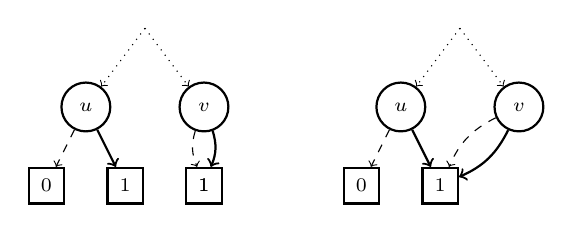
\begin{tikzpicture}[
        bdd/.style={circle, draw, thick, minimum size=0.62cm, inner sep=1pt},
        terminal/.style={rectangle, draw, thick, minimum width=0.45cm, minimum height=0.45cm},
        edge/.style={->, thick},
        every node/.style={font=\scriptsize}
      ]
      \node[bdd] (term_u) at (0.5,1) {\(u\)};
      \node[bdd] (term_v) at (2,1) {\(v\)};
      \node[terminal] (term_0) at (0,0) {0};
      \node[terminal] (term_1) at (1,0) {1};
      \node[terminal] (term_1b) at (2,0) {1};
      \node[terminal] (term_1c) at (2,0) {1};
      \draw[->, dotted] (1.25,2) -- (term_u);
      \draw[->, dotted] (1.25,2) -- (term_v);
      \draw[->, dashed] (term_u) -- (term_0);
      \draw[->, thick] (term_u) -- (term_1);
      \draw[->, dashed] (term_v) to[bend right=20] (term_1b);
      \draw[->, thick] (term_v) to[bend left=20] (term_1c);

      \node at (3,0.5) {\(\implies\)};
      \node[bdd] (term_u2) at (4.5,1) {\(u\)};
      \node[bdd] (term_v2) at (6,1) {\(v\)};
      \node[terminal] (term_02) at (4,0) {0};
      \node[terminal] (term_12) at (5,0) {1};
      \draw[->, dotted] (5.25,2) -- (term_u2);
      \draw[->, dotted] (5.25,2) -- (term_v2);
      \draw[->, dashed] (term_u2) -- (term_02);
      \draw[->, thick] (term_u2) -- (term_12);
      \draw[->, dashed] (term_v2) to[bend right=20] (term_12);
      \draw[->, thick] (term_v2) to[bend left=20] (term_12);
    \end{tikzpicture}
    \caption{Condivisione dei terminali}
  \end{figure}
  \item \keyword{eliminazione dei test ridondanti}: un nodo i cui due archi puntano allo stesso figlio può essere sostituito dal figlio stesso;
  \begin{figure}[H]
    \centering
    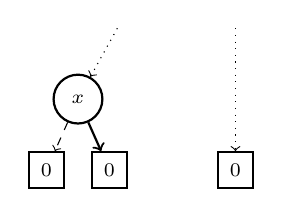
\begin{tikzpicture}[
        bdd/.style={circle, draw, thick, minimum size=0.62cm, inner sep=1pt},
        terminal/.style={rectangle, draw, thick, minimum width=0.45cm, minimum height=0.45cm},
        edge/.style={->, thick},
        every node/.style={font=\scriptsize}
      ]
      \node[bdd] (red_x) at (0,0) {\(x\)};
      \node[terminal] (red_0a) at (-0.4,-0.9) {0};
      \node[terminal] (red_0b) at (0.4,-0.9) {0};
      \draw[->, dotted] (0.5,0.9) -- (red_x);
      \draw[->, dashed] (red_x) -- (red_0a);
      \draw[->, thick] (red_x) -- (red_0b);
      \node at (1.4,0) {\(\implies\)};

        
      \node[terminal] (red_0c) at (2,-0.9) {0};
      \draw[->, dotted] (2,0.9) -- (red_0c);
    \end{tikzpicture}
    \caption{Eliminazione del test ridondante}
  \end{figure}
  \item \keyword{condivisione dei nodi interni}: se due nodi sono radici di sottodiagrammi isomorfi, se ne preserva uno solo, ridirigendo gli archi entranti nell'altro.
  \begin{figure}[H]
    \centering
    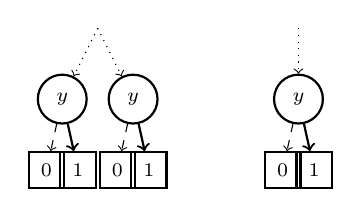
\begin{tikzpicture}[
        bdd/.style={circle, draw, thick, minimum size=0.62cm, inner sep=1pt},
        terminal/.style={rectangle, draw, thick, minimum width=0.45cm, minimum height=0.45cm},
        edge/.style={->, thick},
        every node/.style={font=\scriptsize}
      ]
      \node[bdd] (iso_y1) at (0,0) {\(y\)};
      \node[bdd] (iso_y2) at (0.9,0) {\(y\)};
      \node[terminal] (iso_0a) at (-0.2,-0.9) {0};
      \node[terminal] (iso_1a) at (0.2,-0.9) {1};
      \node[terminal] (iso_0b) at (0.7,-0.9) {0};
      \node[terminal] (iso_1b) at (1.1,-0.9) {1};
      \draw[->, dotted] (0.45,0.9) -- (iso_y1);
      \draw[->, dotted] (0.45,0.9) -- (iso_y2);
      \draw[->, dashed] (iso_y1) -- (iso_0a);
      \draw[->, thick] (iso_y1) -- (iso_1a);
      \draw[->, dashed] (iso_y2) -- (iso_0b);
      \draw[->, thick] (iso_y2) -- (iso_1b);

      \node at (1.8,0) {\(\implies\)};
      \node[bdd] (iso_y3) at (3,0) {\(y\)};
      \node[terminal] (iso_0c) at (2.8,-0.9) {0};
      \node[terminal] (iso_1c) at (3.2,-0.9) {1};
      \draw[->, dotted] (3,0.9) -- (iso_y3);
      \draw[->, dashed] (iso_y3) -- (iso_0c);
      \draw[->, thick] (iso_y3) -- (iso_1c);
    \end{tikzpicture}
    \caption{Condivisione dei nodi interni}
  \end{figure}
\end{itemize}

\begin{observation}{Località del test di isomorfismo}
  Il test di isomorfismo può sembrare costoso, perché sembrerebbe richiedere il confronto di interi sottodiagrammi. Ma se le regole si applicano dal basso verso l'alto, il test diventa \emph{locale}: due nodi sono radici di sottodiagrammi isomorfi se e solo se hanno la stessa etichetta e archi basso e alto che puntano rispettivamente agli stessi nodi. Infatti, se i sottodiagrammi dei figli erano isomorfi, sono già stati unificati da applicazioni precedenti della regola.
\end{observation}

\begin{example}{Trasformazione da Decision Tree a BDD}
  Vediamo dunque un esempio di trasformazione da albero di decisione a BDD, applicando le regole di riduzione. Consideriamo la banale funzione \(f(x,y,z) = x \lor (y\land z)\), il cui albero di decisione è:
  \begin{figure}[H]
    \centering
    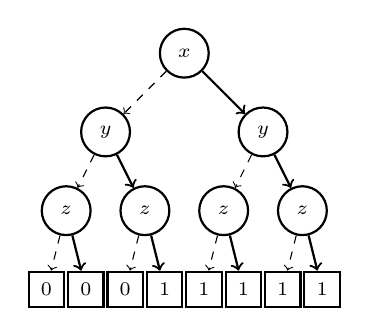
\begin{tikzpicture}[
        bdd/.style={circle, draw, thick, minimum size=0.62cm, inner sep=1pt},
        terminal/.style={rectangle, draw, thick, minimum width=0.45cm, minimum height=0.45cm},
        edge/.style={->, thick},
        every node/.style={font=\scriptsize}
      ]
      \node[bdd] (x) at (0,0) {\(x\)};
      \node[bdd] (y1) at (-1,-1) {\(y\)};
      \node[bdd] (y2) at (1,-1) {\(y\)};
      \node[bdd] (z1) at (-1.5,-2) {\(z\)};
      \node[bdd] (z2) at (-0.5,-2) {\(z\)};
      \node[bdd] (z3) at (0.5,-2) {\(z\)};
      \node[bdd] (z4) at (1.5,-2) {\(z\)};
      \node[terminal] (t0) at (-1.75,-3) {0};
      \node[terminal] (t1) at (-1.25,-3) {0};
      \node[terminal] (t2) at (-0.75,-3) {0};
      \node[terminal] (t3) at (-0.25,-3) {1};
      \node[terminal] (t4) at (0.25,-3) {1};
      \node[terminal] (t5) at (0.75,-3) {1};
      \node[terminal] (t6) at (1.25,-3) {1};
      \node[terminal] (t7) at (1.75,-3) {1};
      \draw[->, dashed] (x) -- (y1);
      \draw[->, thick] (x) -- (y2);
      \draw[->, dashed] (y1) -- (z1);
      \draw[->, thick] (y1) -- (z2);
      \draw[->, dashed] (y2) -- (z3);
      \draw[->, thick] (y2) -- (z4);
      \draw[->, dashed] (z1) -- (t0);
      \draw[->, thick] (z1) -- (t1);
      \draw[->, dashed] (z2) -- (t2);
      \draw[->, thick] (z2) -- (t3);
      \draw[->, dashed] (z3) -- (t4);
      \draw[->, thick] (z3) -- (t5);
      \draw[->, dashed] (z4) -- (t6);
      \draw[->, thick] (z4) -- (t7);
    \end{tikzpicture}
    \caption{Albero di decisione per \(f(x,y,z) = x \lor (y\land z)\)}
  \end{figure}
  Applichiamo ora le regole di riduzione, dal basso verso l'alto:
  \begin{figure}[H]
    \centering
    \begin{minipage}{0.3\textwidth}

      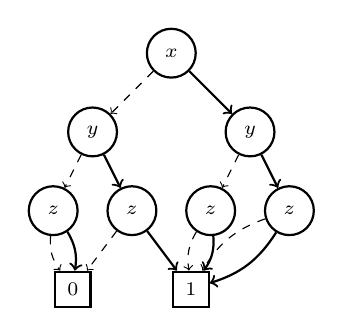
\begin{tikzpicture}[
        bdd/.style={circle, draw, thick, minimum size=0.62cm, inner sep=1pt},
        terminal/.style={rectangle, draw, thick, minimum width=0.45cm, minimum height=0.45cm},
        edge/.style={->, thick},
        every node/.style={font=\scriptsize}
        ]
      \node[bdd] (x) at (0,0) {\(x\)};
      \node[bdd] (y1) at (-1,-1) {\(y\)};
      \node[bdd] (y2) at (1,-1) {\(y\)};
      \node[bdd] (z1) at (-1.5,-2) {\(z\)};
      \node[bdd] (z2) at (-0.5,-2) {\(z\)};
      \node[bdd] (z3) at (0.5,-2) {\(z\)};
      \node[bdd] (z4) at (1.5,-2) {\(z\)};
      \node[terminal] (t0) at (-1.25,-3) {0};
      \node[terminal] (t1) at (0.25,-3) {1};
      \draw[->, dashed] (x) -- (y1);
      \draw[->, thick] (x) -- (y2);
      \draw[->, dashed] (y1) -- (z1);
      \draw[->, thick] (y1) -- (z2);
      \draw[->, dashed] (y2) -- (z3);
      \draw[->, thick] (y2) -- (z4);
      \draw[->, dashed] (z1) to[bend right=20] (t0);
      \draw[->, thick] (z1) to[bend left=20] (t0);
      \draw[->, dashed] (z2) -- (t0);
      \draw[->, thick] (z2) -- (t1);
      \draw[->, dashed] (z3) to[bend right=20] (t1);
      \draw[->, thick] (z3) to[bend left=20] (t1);
      \draw[->, dashed] (z4) to[bend right=20] (t1);
      \draw[->, thick] (z4) to[bend left=20] (t1);
    \end{tikzpicture}
  \end{minipage}
  \begin{minipage}{0.3\textwidth}
      
      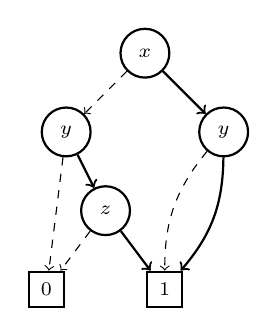
\begin{tikzpicture}[
        bdd/.style={circle, draw, thick, minimum size=0.62cm, inner sep=1pt},
        terminal/.style={rectangle, draw, thick, minimum width=0.45cm, minimum height=0.45cm},
        edge/.style={->, thick},
        every node/.style={font=\scriptsize}
        ]
      \node[bdd] (x) at (0,0) {\(x\)};
      \node[bdd] (y1) at (-1,-1) {\(y\)};
      \node[bdd] (y2) at (1,-1) {\(y\)};
      \node[bdd] (z2) at (-0.5,-2) {\(z\)};
      \node[terminal] (t0) at (-1.25,-3) {0};
      \node[terminal] (t1) at (0.25,-3) {1};
      \draw[->, dashed] (x) -- (y1);
      \draw[->, thick] (x) -- (y2);
      \draw[->, dashed] (y1) -- (t0);
      \draw[->, thick] (y1) -- (z2);
      \draw[->, dashed] (y2) to[bend right=20] (t1);
      \draw[->, thick] (y2) to[bend left=20] (t1);

      \draw[->, dashed] (z2) -- (t0);
      \draw[->, thick] (z2) -- (t1);

    \end{tikzpicture}
  \end{minipage}
  \begin{minipage}{0.3\textwidth}
      
      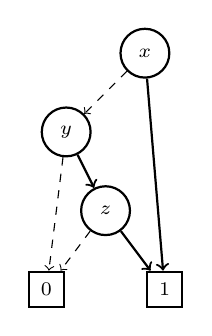
\begin{tikzpicture}[
        bdd/.style={circle, draw, thick, minimum size=0.62cm, inner sep=1pt},
        terminal/.style={rectangle, draw, thick, minimum width=0.45cm, minimum height=0.45cm},
        edge/.style={->, thick},
        every node/.style={font=\scriptsize}
        ]
     \node[bdd] (x) at (0,0) {\(x\)};
      \node[bdd] (y1) at (-1,-1) {\(y\)};
      \node[bdd] (z2) at (-0.5,-2) {\(z\)};
      \node[terminal] (t0) at (-1.25,-3) {0};
      \node[terminal] (t1) at (0.25,-3) {1};
      \draw[->, dashed] (x) -- (y1);
      \draw[->, thick] (x) -- (t1);
      \draw[->, dashed] (y1) -- (t0);
      \draw[->, thick] (y1) -- (z2);

      \draw[->, dashed] (z2) -- (t0);
      \draw[->, thick] (z2) -- (t1);

    \end{tikzpicture}
  \end{minipage}
  \caption{Riduzione dell'albero di decisione a BDD}
  \end{figure}
\end{example}

\section{OBDD: ordinamento e canonicità}

La rappresentazione BDD non è ancora canonica: per la stessa funzione è possibile scegliere una qualsiasi variabile per etichettare il nodo iniziale, ottenendo BDD completamente diversi; in linea di principio ogni ordinamento dei test porta a un grafo diverso. La forma canonica si ottiene fissando un ordinamento sulle variabili.

\begin{definition}{OBDD}
  Fissato un ordinamento totale \(x_1 \prec x_2 \prec \cdots \prec x_n\) sulle variabili, un \keyword{Ordered BDD} (OBDD) è un BDD in cui, su ogni percorso dal nodo iniziale ai terminali, le variabili compaiono rispettando l'ordinamento.
\end{definition}

\begin{theorem}{Canonicità}
  Fissato l'ordinamento sulle variabili, per ogni funzione booleana esiste un unico OBDD ridotto (ROBDD) che la rappresenta.
\end{theorem}

La canonicità è la proprietà chiave: il test di uguaglianza tra funzioni (e dunque tra insiemi, rappresentati dalle loro funzioni caratteristiche) si riduce a un test di isomorfismo tra OBDD, eseguibile in tempo lineare nelle dimensioni. In pratica si fa ancora meglio: l'eliminazione della ridondanza si applica all'intera \emph{foresta} di BDD di tutte le funzioni in uso, ammettendo più radici in un unico DAG condiviso. In questo modo due funzioni equivalenti fanno riferimento allo stesso oggetto, e la verifica di uguaglianza diventa costante: basta confrontare gli identificativi (puntatori).

\subsection{L'importanza dell'ordinamento}

L'ordine delle variabili non è importante solo per la canonicità, ma anche per la \emph{dimensione} del diagramma.

\begin{example}{}
  Consideriamo la funzione \(f = \bigwedge_{i=1}^n (x_i \leftrightarrow y_i)\). Con l'ordinamento \(x_1,y_1,x_2,y_2,\dots,x_n,y_n\) (variabili correlate adiacenti), l'OBDD ha dimensione \(3n + 2\), lineare. Con l'ordinamento \(x_1,x_2,\ldots, x_n,y_1,y_2, \ldots, y_n\), invece, la dimensione è \(3\cdot 2^n-1\), esponenziale.
  \begin{figure}[H]
      \centering
      \tikzset{
          bddnode/.style={circle, draw, minimum size=7mm, inner sep=0pt, font=\small},
          terminal/.style={rectangle, draw, minimum size=6mm, font=\small\bfseries},
          edge0/.style={->, dashed, thick},
          edge1/.style={->, solid, thick}
      }
      
      % PRIMO GRAFO: Ordinamento Lineare
      \begin{minipage}{0.45\textwidth}
          \centering
          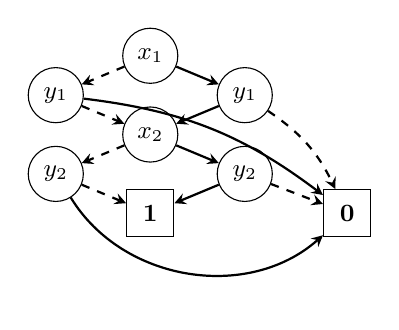
\begin{tikzpicture}[>=stealth]
              % Nodi variabili
              \node[bddnode] (x1) at (0, 0) {\(x_1\)};
              
              \node[bddnode] (y1L) at (-1.2, -0.5) {\(y_1\)};
              \node[bddnode] (y1R) at (1.2, -0.5) {\(y_1\)};
              
              \node[bddnode] (x2) at (0, -1) {\(x_2\)};
              
              \node[bddnode] (y2L) at (-1.2, -1.5) {\(y_2\)};
              \node[bddnode] (y2R) at (1.2, -1.5) {\(y_2\)};
              
              % Terminali
              \node[terminal] (T1) at (0, -2) {1};
              \node[terminal] (T0) at (2.5, -2) {0};
              
              % Archi (edge0 = tratteggiato/falso, edge1 = solido/vero)
              \draw[edge0] (x1) -- (y1L);
              \draw[edge1] (x1) -- (y1R);
              
              \draw[edge0] (y1L) -- (x2);
              \draw[edge1] (y1L) to[bend left=15] (T0);
              
              \draw[edge0] (y1R) to[bend left=15] (T0);
              \draw[edge1] (y1R) -- (x2);
              
              \draw[edge0] (x2) -- (y2L);
              \draw[edge1] (x2) -- (y2R);
              
              \draw[edge0] (y2L) -- (T1);
              \draw[edge1] (y2L) to[bend right=50] (T0);
              
              \draw[edge0] (y2R) -- (T0);
              \draw[edge1] (y2R) -- (T1);
          \end{tikzpicture}
          \caption*{Ordine \(x_1, y_1, x_2, y_2\) (Dim: 8)}
      \end{minipage}\hfill
      % SECONDO GRAFO: Ordinamento Esponenziale
      \begin{minipage}{0.5\textwidth}
          \centering
          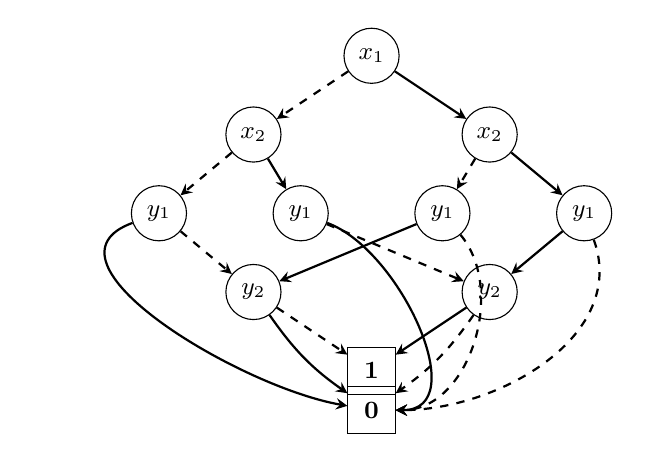
\begin{tikzpicture}[>=stealth]
              % Livello x1
              \node[bddnode] (x1) at (0, 0) {\(x_1\)};
              
              % Livello x2
              \node[bddnode] (x2L) at (-1.5, -1) {\(x_2\)};
              \node[bddnode] (x2R) at (1.5, -1) {\(x_2\)};
              
              % Livello y1 (4 nodi per memorizzare le combinazioni di x1, x2)
              \node[bddnode] (y1_00) at (-2.7, -2) {\(y_1\)};
              \node[bddnode] (y1_01) at (-0.9, -2) {\(y_1\)};
              \node[bddnode] (y1_10) at (0.9, -2) {\(y_1\)};
              \node[bddnode] (y1_11) at (2.7, -2) {\(y_1\)};
              
              % Livello y2
              \node[bddnode] (y2_0) at (-1.5, -3) {\(y_2\)};
              \node[bddnode] (y2_1) at (1.5, -3) {\(y_2\)};
              
              % Terminali
              \node[terminal] (T1) at (0, -4) {1};
              \node[terminal] (T0) at (0, -4.5) {0};
              
              % Archi x1 -> x2
              \draw[edge0] (x1) -- (x2L);
              \draw[edge1] (x1) -- (x2R);
              
              % Archi x2 -> y1
              \draw[edge0] (x2L) -- (y1_00);
              \draw[edge1] (x2L) -- (y1_01);
              \draw[edge0] (x2R) -- (y1_10);
              \draw[edge1] (x2R) -- (y1_11);
              
              % Archi y1 -> y2 / T0
              \draw[edge0] (y1_00) -- (y2_0);
              \draw[edge1] (y1_00) to[out=200, in=170] (T0);
              
              \draw[edge0] (y1_01) -- (y2_1);
              \draw[edge1] (y1_01) to[out=340, in=0] (T0);
              
              \draw[edge0] (y1_10) to[out=310, in=0] (T0);
              \draw[edge1] (y1_10) -- (y2_0);
              
              \draw[edge0] (y1_11) to[out=290, in=0] (T0);
              \draw[edge1] (y1_11) -- (y2_1);
              
              % Archi y2 -> Terminali
              \draw[edge0] (y2_0) -- (T1);
              \draw[edge1] (y2_0) to[bend right=10] (T0);
              
              \draw[edge0] (y2_1) to[bend left=10] (T0);
              \draw[edge1] (y2_1) -- (T1);
          \end{tikzpicture}
          \caption*{Ordine \(x_1, x_2, y_1, y_2\) (Dim: 11)}
      \end{minipage}
      \vspace{0.3cm}
      \caption*{Esempio visivo per \(n=2\).}
  \end{figure}
\end{example}

Sfortunatamente funzioni diverse hanno ordinamenti ottimali diversi, e decidere qual è l'ordinamento ottimale è un problema NP-completo. Nella pratica vengono adottate euristiche, senza però garanzia di ottenere OBDD compatti.

\begin{warning}{}
  Esistono funzioni (legate ad esempio alla moltiplicazione binaria) il cui OBDD è esponenziale per \emph{qualsiasi} ordinamento: la rappresentazione simbolica non è una bacchetta magica, e i collegamenti con SAT e VALIDITY (che su OBDD canonici si risolvono in tempo costante, guardando se l'OBDD è diverso da \(0\) o uguale a \(1\)) implicano che il costo esponenziale si scarica sulla \emph{costruzione} dell'OBDD.
\end{warning}

Applicando le regole di riduzione a un albero di decisione si ottiene un OBDD ridotto, o \keyword{ROBDD}.

\begin{definition}{ROBDD}
  Un \keyword{Reduced OBDD} (ROBDD) è un OBDD tale che:
  \begin{enumerate}
    \item esistono esattamente due vertici terminali, etichettati rispettivamente con \(1\) e \(0\);
    \item \[\forall v \in V, low(v)\neq high(v)\]
    \item \[\forall u,v \in V, low(u) = low(v) \land high(u) = high(v) \land var(u) = var(v) \implies u = v\]
  \end{enumerate}
\end{definition}

\subsection{Costruzione dei ROBDD}

Le regole di riduzione della obdd-canonicity descrivono \emph{quando} un BDD è ridondante, ma non dicono come costruire direttamente un OBDD già ridotto. L'approccio ingenuo — costruire prima l'intero albero di decisione e poi applicare le regole di riduzione dal basso verso l'alto, come sulla località del test di isomorfismo — funziona, ma è inutilmente costoso: l'albero di decisione completo ha sempre \(2^{n+1}-1\) nodi, indipendentemente da quanto l'OBDD finale sia piccolo. Vogliamo invece un procedimento che produca nodi \emph{già canonici}, senza mai passare per la rappresentazione intermedia esponenziale.

L'idea è mantenere \emph{due} tabelle, che rappresentano lo stesso insieme di nodi indicizzato in due modi complementari:
\begin{itemize}
  \item la \keyword{tabella del grafo} \(T\), indicizzata per identificatore di nodo, che associa a ogni nodo \(u\) la sua tripla \((var(u), low(u), high(u))\): è la rappresentazione del DAG vero e proprio, quella che si attraversa per valutare la funzione;
  \item la \keyword{tabella di hashing} \(H\) (o \emph{unique table}), indicizzata per tripla, che associa a \((x,l,h)\) l'identificatore del nodo con quella struttura, \emph{se già esiste}.
\end{itemize}
Le due tabelle sono l'una l'inversa dell'altra: \(T[u] = (x,l,h) \iff H[(x,l,h)] = u\). Servono entrambe le direzioni perché durante la costruzione bisogna sia navigare il DAG a partire da un nodo (\(T\)), sia chiedersi, prima di creare un nodo nuovo, se una struttura equivalente esiste già (\(H\)) — ed è proprio quest'ultimo controllo, se implementato con una tabella hash, a rendere il test in tempo atteso costante anziché lineare nel numero di nodi già creati.

\begin{algorithmdesc}{Creazione canonica di un nodo}
  \begin{algorithmic}[1]
    \Statex{} \textbf{signature} \(\textsc{Mk:} \quad Var \times NodeId \times NodeId \to NodeId\)
    \Function{\(\textsc{Mk}\)}{$x,l,h$} % chktex 46
    \If{\(l = h\)}
    \State{} \Return{} \(l\)
    \ElsIf{\((x,l,h) \in \mathrm{dom}(H)\)}
    \State{} \Return{} \(H[(x,l,h)]\)
    \Else{}
    \State{} \(u \gets FreshNodeId()\) \Comment{} ottieni un nuovo identificatore di nodo
    \State{} \(T[u] \gets (x,l,h)\)
    \State{} \(H[(x,l,h)] \gets u\)
    \State{} \Return{} \(u\)
    \EndIf{}
    \EndFunction{}
  \end{algorithmic}
\end{algorithmdesc}

La funzione \(\textsc{Mk}\) è l'\emph{unico} punto del procedimento in cui vengono creati nodi, e applica in un solo passaggio entrambe le regole di riduzione strutturale già viste: la condizione \(l=h\) è esattamente l'eliminazione dei test ridondanti (un nodo i cui due archi portano allo stesso figlio collassa nel figlio stesso, senza bisogno di distinguere il valore di \(x\)); il controllo su \(H\) è la condivisione dei nodi interni, e garantisce che due sottodiagrammi con struttura identica restino un unico nodo condiviso in memoria, mai duplicato. La condivisione dei terminali, invece, è garantita a monte: i nodi \(0\) e \(1\) vengono creati una sola volta in fase di inizializzazione e riutilizzati sempre come possibili valori di \(l,h\).

\begin{note}{}
  Chiamare \(\textsc{Mk}\) al posto di creare direttamente un nuovo nodo è ciò che rende l'intero procedimento canonico \emph{per costruzione}: non serve mai un passaggio separato di riduzione a posteriori, perché ogni nodo, nel momento stesso in cui viene richiesto, o riusa una struttura già presente o ne crea esattamente una, mai più di una, per ogni tripla distinta.
\end{note}

Con \(\textsc{Mk}\) a disposizione, la costruzione dell'OBDD di una funzione booleana \(f\) sulle variabili ordinate \(x_1 \prec \cdots \prec x_n\) procede seguendo esattamente l'espansione di Shannon: si calcolano ricorsivamente i due cofattori rispetto alla variabile corrente, si costruiscono i loro OBDD sulle variabili rimanenti, e li si richiude con \(\textsc{Mk}\).

\begin{algorithmdesc}{Build: costruzione dell'OBDD di una funzione}
  \begin{algorithmic}[1]
    \Statex{} \textbf{signature} \(\textsc{Build:} \quad BoolFun \times \mathbb{N} \to NodeId\)
    \Function{\(\textsc{Build}\)}{$f,i$} % chktex 46
    \If{\(i \succ n\)}
    \State{} \Return{} \(Terminal(1)\) se \(f \equiv 1\), \(Terminal(0)\) se \(f \equiv 0\)
    \Else{}
    \State{} \(v_0 \gets \textsc{Build}(f_{\overline{x_i}}, i+1)\)
    \State{} \(v_1 \gets \textsc{Build}(f_{x_i}, i+1)\)
    \State{} \Return{} \(\textsc{Mk}(x_i, v_0, v_1)\)
    \EndIf{}
    \EndFunction{}
  \end{algorithmic}
\end{algorithmdesc}

La correttezza si dimostra per induzione, procedendo dall'ultima variabile alla prima: se \(v_0\) e \(v_1\) sono già i ROBDD canonici dei rispettivi cofattori (base dell'induzione: i terminali sono banalmente canonici), allora \(\textsc{Mk}(x_i,v_0,v_1)\) restituisce il ROBDD canonico di \(f\), per lo stesso argomento di canonicità-per-costruzione appena discusso.

\begin{observation}{Complessità di Build}
  Così come presentato, \(\textsc{Build}\) nel caso peggiore effettua \(\BigO{2^n}\) chiamate ricorsive: una per ogni possibile assegnamento delle variabili, esattamente come nella costruzione dell'albero di decisione completo, perché i cofattori vengono ricalcolati indipendentemente lungo ogni ramo, senza alcuna cache sulle chiamate ricorsive stesse (solo \(\textsc{Mk}\) è cached, tramite \(H\)). Quello che si può fare è memorizzare i risultati parziali di \(\textsc{Build}\) in una tabella indicizzata da \((f,i)\), così che ogni coppia distinta venga calcolata una sola volta. In questo modo la complessità totale diventa \(\BigO{\abs{f}}\), dove \(\abs{f}\) è la dimensione dell'OBDD finale.
\end{observation}


\section{Operazioni sugli OBDD}

Per il model checking simbolico servono le operazioni insiemistiche (\(\cap, \cup\), complemento) sulle funzioni caratteristiche, e la preimmagine. Vediamo come implementarle.

\subsection{L'algoritmo Apply}

Dati gli OBDD di due funzioni \(f\) e \(g\), vogliamo calcolare l'OBDD di \(f \circ g\) per un operatore booleano binario \(\circ\). L'idea sfrutta il fatto che l'espansione di Shannon commuta con gli operatori booleani:
\begin{equation*}
  \begin{aligned}
    f \lor g & = ((x_1 \land f_{x_1}) \lor (\neg x_1 \land f_{\overline{x_1}})) \lor ((x_1 \land g_{x_1}) \lor (\neg x_1 \land g_{\overline{x_1}})) \\
             & = (x_1 \land (f_{x_1} \lor g_{x_1})) \lor (\neg x_1 \land (f_{\overline{x_1}} \lor g_{\overline{x_1}}))
  \end{aligned}
\end{equation*}
e lo stesso vale per \(\land\) e per la negazione (esprimibile come \(\neg f \equiv f \oplus 1 \equiv\)). Possiamo facilmente notare in oltre che, se \(f\) e \(g\) differiscono nella loro prima variabile discriminante, l'espansione di Shannon si applica solo a quella variabile, lasciando invariata l'altra funzione. In altre parole, la ricorsione scende solo sui sottoalberi che dipendono dalla variabile corrente. Infine, il caso base non è altro che rappresentato dall'applicazione dell'operatore booleano ai due valori terminali.

\begin{note}{Costruzione di ROBDD senza algoritmo Build}
  L'algoritmo \textsc{Apply} fornisce un metodo alternativo per costruire l'OBDD di una funzione booleana a partire da due funzioni più semplici, senza passare per la costruzione dell'albero di decisione completo. In particolare, se \(f\) e \(g\) sono già OBDD canonici, allora \(\textsc{Apply}(f,g,\circ)\) restituisce l'OBDD canonico di \(f \circ g\).
\end{note}

\todo[inline]{Aggiungere lo pseudocodice dell'algoritmo Apply dalle slide}

\begin{algorithmdesc}{Apply: operazioni binarie sugli OBDD}
  \begin{algorithmic}[1]
    \Statex{} \textbf{signature} \(\textsc{Apply:} \quad BoolOp \times NodeId \times NodeId \to NodeId\)
    \Function{\(\textsc{Apply}\)}{$\circ,u,v$} %chktex 46
      \Function{\(TerminalCase\)}{$\circ,u,v$} %chktex 46
        \If{\(isTerminal(u) \land isTerminal(v)\)}
          \State{} \Return{} \(True\)
        \EndIf{}
        \If{\(\circ = \land\)}
          \State{} \Return{} \(u = Terminal(0) \lor v = Terminal(0)\)
        \ElsIf{\(\circ = \lor\)}
          \State{} \Return{} \(u = Terminal(1) \lor v = Terminal(1)\)
        \ElsIf{\(\circ = \oplus\)}
          \State{} \Return{} \(u = Terminal(0) \lor v = Terminal(0) \lor v=u\)
        \EndIf{}
      \EndFunction{}
      \Function{\(\textsc{App}\)}{$u,v$} %chktex 46
        \If{\(TerminalCase(\circ,u,v)\)}
          \State{} \Return{} \(\circ(u,v)\) \Comment{} \(\circ\) è a corto circuito
        \EndIf{}
        \State{} \(low_u, high_u \gets u,u\)
        \State{} \(low_v, high_v \gets v,v\)
        \State{} \(var \gets var(u)\)
        \If{\(var(u) \leq var(v)\)}
          \State{} \(low_u, high_u \gets low(u), high(u)\)
        \EndIf{}
        \If{\(var(v) \leq var(u)\)}
          \State{} \(low_v, high_v \gets low(v), high(v)\)
          \State{} \(var \gets var(v)\)
        \EndIf{}
        \State{} \Return{} \(\textsc{Mk}(var, \textsc{App}(low_u, low_v), \textsc{App}(high_u, high_v))\)
      \EndFunction{}
      \State{} \Return{} \(\textsc{App}(u,v)\)
    \EndFunction{}
  \end{algorithmic}
  
\end{algorithmdesc}


\begin{note}{}
  Nei casi in cui uno dei due OBDD dipende da una variabile da cui l'altro non dipende, la ricorsione scende solo su quello che ne dipende, lasciando l'altro invariato.
\end{note}

L'algoritmo di base ha complessità \(\BigO{2^n}\), perché ripete più volte le stesse chiamate ricorsive. Il problema si risolve con programmazione dinamica: mantenendo una cache dei risultati parziali indicizzata dalle triple \((\circ,u,v)\), ogni chiamata ricorsiva viene eseguita una sola volta e le successive risolte con un lookup a tempo costante. Fissato \(\circ\), le chiamate distinte sono al più \(\abs{f}\cdot \abs{g}\), e dunque la complessità totale è \(\BigO{\abs{f}\cdot \abs{g}}\).

\subsection{Restrizione e quantificazione booleana}

Data \(f(x_1,\ldots,x_n)\), la \keyword{restrizione} rispetto a un assegnamento parziale calcola l'OBDD dei cofattori, ad esempio \(f_{x_i}\) e \(f_{\overline{x_i}}\). Anche questa operazione può essere riformulata in funzione di espansione di Shannon, ma non essendo un operazione binaria, non è direttamente implementabile con \textsc{Apply}.

La restrizione è particolarmente utile per le \keyword{Quantified Boolean Formulae} (QBF), formule booleane quantificate con semantica identica al prim'ordine su dominio booleano. Dal punto di vista funzionale:
\[\exists x_i.\, f(x_1, \ldots, x_n) \equiv f_{x_i} \lor f_{\overline{x_i}} \qquad \forall x_i.\, f(x_1, \ldots, x_n) \equiv f_{x_i} \land f_{\overline{x_i}}\]

Dunque utilizzando \textsc{Apply} con \(\lor\) e \(\land\) appropriatamente sulle restrizioni, è possibile implementare la quantificazione booleana.

Per il model checking simbolico di \(CTL\) sarà sufficiente \(\exists\) per la preimmagine, che è intrinsecamente una proprietà esistenziale. In contesti di logica alternante invece, come nei giochi visti nel \Cref{ch:atl}, la preimmagine può invece essere universale, richiedendo entrambe le restrizioni.

Per l'implementazione della restrizione diretta sugli OBDD possiamo analizzare la loro struttura ricorsiva. Sia \(y\) la variabile da fissare a \(1\) o \(0\), e sia \(f\) l'OBDD della funzione booleana con variabile iniiziale \(x\). Per calcolare \(f_y\) o \(f_{\overline{y}}\) è sufficiente analizzare la posizione di \(y\) rispetto alla variabile del nodo corrente \(x\), in particolare:
\begin{itemize}
  \item Se \(y = x\), allora la riduzione si risolve immediatamente: \(f_y = high(f)\) e \(f_{\overline{y}} = low(f)\);
  \item Se \(y \prec x\), allora \(y\) non compare in \(f\), e dunque \(f_y = f_{\overline{y}} = f\);
  \item Se \(y \succ x\), allora la riduzione si applica ricorsivamente ai due figli: \(f_y = x\to high(f)_y ,low(f)_y\) e \(f_{\overline{y}} = x\to high(f)_{\overline{y}} ,low(f)_{\overline{y}}\).
\end{itemize}

Algoritmicamente il terzo caso è implementabile tramite due chiamate ricorsive su \(high(f)\) e \(low(f)\) rispettivamente.

\begin{algorithmdesc}{Restrict: calcolo della restrizione di un OBDD}
  \begin{algorithmic}[1]
    \Statex{} \textbf{signature} \(\textsc{Restrict:} \quad NodeId \times Var \times Bool \to NodeId\)
    \Function{\(\textsc{Restrict}\)}{$f,y,b$} %chktex 46
      \If{\(isTerminal(f)\)}
        \State{} \Return{} \(f\)
      \EndIf{}
      \Function{\(Res\)}{$f$} %chktex 46
        \If{\(var(f) \succ i\)}
          \State{} \Return{} \(f\)
        \ElsIf{\(var(f) \prec i\)}
          \State{} \Return{} \(\textsc{Mk}(var(f), Res(low(f)), Res(high(f)))\)
        \Else{}\Comment{} \(var(f) = i\)
          \If{\(b = 0\)}
            \State{} \Return{} \(Res(low(f))\)
          \Else{}
            \State{} \Return{} \(Res(high(f))\)
          \EndIf{}
        \EndIf{}
      \EndFunction{}
      \State{} \Return{} \(Res(f)\)
    \EndFunction{}
  \end{algorithmic}
\end{algorithmdesc}

Anche in questo caso questa versione dell'algoritmo risulta essere esponenziale, ma utilizzando una cache per memorizzare i risultati parziali, la complessità diventa lineare nella dimensione dell'OBDD di partenza.

\section{Model checking simbolico di CTL}
Abbiamo tutti gli ingredienti per il model checking simbolico. L'input è una struttura di Kripke: dobbiamo capire come codificarne la topologia tramite OBDD\@.

\subsection{Codifica di stati e transizioni}
Sia \(K = (AP,S,S_0,R,\lambda)\) una struttura di Kripke, con \(S = \{s_1, \ldots, s_m\}\) e \(AP = \{p_1, \ldots, p_n\}\). Ogni stato \(s_i\) è etichettato da un sottoinsieme di proposizioni atomiche: \(\lambda(s_i) \subseteq AP\). Possiamo rappresentare ogni stato come un assegnamento booleano alle variabili \(x_1, \ldots, x_n\), dove \(x_j = 1\) se e solo se \(p_j \in \lambda(s_i)\). In altre parole, ogni stato è rappresentato dalla sua funzione caratteristica:
\[\forall s_i \in S: f_{s_i} = \bigwedge_{p_j \in \lambda(s_i)} x_j \land \bigwedge_{p_j \notin \lambda(s_i)} \neg x_j\]
tale rappresentazione è sufficiente anche per rappresentare il singleton di ogni stato, permettendo di rappresentare ogni insieme di stati \(S'\subseteq S\) come la disgiunzione delle funzioni caratteristiche dei singoli stati che lo compongono:
\[\forall S' \subseteq S: f_{S'} = \bigvee_{s_i \in S'} f_{s_i}\]

Tale costruzione assume che \(\lambda\) sia iniettiva, ovvero che stati diversi abbiano etichettature diverse.Se così non fosse, basterebbe aggiungere qualche proposizione atomica fresca per distinguerli.

Di conseguenza, si ha che \(S \subseteq 2^{AP}\), e dunque \(\abs{S} \leq 2^n\). In oltre, essendo \(R \subseteq S \times S\), si ha che \(\abs{R} \leq 2^{2n}\). Di conseguenza tale rappresentazione, pur rimanendo lineare nella dimensione del grafo sottostante alla struttura di Kripke, rischia di essere esponenziale nel numero di proposizioni atomiche. In pratica, però, casi reali hanno una struttura molto regolare, e la rappresentazione simbolica tramite OBDD è spesso molto più compatta della rappresentazione esplicita.

Per la relazione di transizione \(R\subseteq S\times S\), avendo già la rappresentazione degli stati con le variabili \(x_1, \ldots, x_{n}\), è sufficiente raddoppiare le variabili introducendo \(x_1', \ldots, x_{n}'\) (\keyword{variabili primate}) e costruire un OBDD \(f_R\) che dipende da entrambe le sequenze: le variabili non primate rappresentano lo stato di partenza, quelle primate lo stato di arrivo. Se ad esempio \((s_1,s_2)\in R\), con \(L(s_1)=\{p,q\}\) e \(L(s_2)=\{r\}\), il termine corrispondente è
\[f_R(s_1,s_2) = f_{s_1}\land f'_{s_2} = (p\land q\land\neg r)\land(p'\land q'\land\neg r')\]
e \(f_R\) è l'OR di questi termini su tutte le coppie in \(R\):
\[f_R = \bigvee_{(s_1,s_2)\in R} f_R(s_1,s_2)\]

\begin{example}{}
  Consideriamo una struttura di Kripke con \(AP= \{p,q,r,t\}\), \(S = \{s_1, s_2, s_3\}\) e \(R = \{(s_1,s_2), (s_1,s_3), (s_2,s_1), (s_3,s_3)\}\). Fissando una codifica posizionale, la rappresentazione booleana dei singoli stati è:
  \begin{align*}
    f_{s_1} & = p \land q \land \neg r \land \neg t \\
    f_{s_2} & = p \land \neg q \land r \land \neg t \\
    f_{s_3} & = \neg p \land \neg q \land r \land t
  \end{align*}
  La relazione di transizione globale \(f_R\) si ottiene come disgiunzione delle transizioni puntuali, affiancando le variabili di stato corrente a quelle di stato successivo (\(v'\)):
  \begin{align*}
    f_R & = (f_{s_1} \land f'_{s_2}) \lor (f_{s_1} \land f'_{s_3}) \lor (f_{s_2} \land f'_{s_1}) \lor (f_{s_3} \land f'_{s_3}) \\
        & = (p \land q \land \neg r \land \neg t \land p' \land \neg q' \land r' \land \neg t') \lor\\
        & \quad (p \land q \land \neg r \land \neg t \land \neg p' \land \neg q' \land r' \land t') \lor \\
        & \quad (p \land \neg q \land r \land \neg t \land p' \land q' \land \neg r' \land \neg t') \lor \\
        & \quad (\neg p \land \neg q \land r \land t \land \neg p' \land \neg q' \land r' \land t')
  \end{align*}

  Sebbene in questo esempio didattico la formula espliciti tutti i 32 letterali corrispondenti ai 4 archi del grafo, la rappresentazione in memoria tramite OBDD opererà una drastica riduzione spaziale. Utilizzando un ordinamento di \emph{interleaving} delle variabili (\(p \prec p' \prec q \prec q' \dots\)), il processo di riduzione dell'OBDD identificherà e fonderà i sotto-grafi isomorfi. Ad esempio, i fattori comuni ricorrenti come la transizione \((\neg t \land \neg t')\) condivisa dai primi tre archi, verranno rappresentati da un unico percorso nel grafo decisionale, dimostrando la capacità della struttura simbolica di astrarre e comprimere le regolarità del modello rispetto a un'enumerazione esplicita in memoria.

\end{example}

\begin{note}{}
  Per l'ordinamento conviene alternare ogni variabile con la sua primata (\(x_1 \prec x_1' \prec x_2 \prec x_2' \prec \cdots\)), essendo strettamente correlate: come visto nell'esempio sull'ordinamento, tenere lontane variabili correlate fa esplodere la dimensione dell'OBDD\@.
\end{note}

\subsection{L'algoritmo simbolico}
Costruiamo induttivamente l'OBDD della denotazione \(\den{\phi}\) di ogni sottoformula:
\begin{itemize}
  \item per le proposizioni atomiche, \(\den{p_i}=f_{p_i}(x_1,\ldots,x_n)=x_i\) è l'OBDD della variabile corrispondente;
  \item per gli operatori booleani, si applica \textsc{Apply} con l'operatore corrispondente agli OBDD delle sottoformule: \(\den{\neg\phi}=f_{\phi}\oplus 1\), \(\den{\phi\land\psi}=f_{\phi}\land f_{\psi}\), e analogamente per \(\lor\);
  \item per \(EX\phi\), serve la preimmagine simbolica (detta anche \keyword{relational product}): si prende \(f_{\phi}(x_1,\ldots,x_n)\), la si \emph{rinomina} sulle variabili primate ottenendo \(f_{\phi}(x_1', \ldots, x_n')\) (in modo da interpretarla sugli stati di arrivo), la si interseca con \(f_{R}\), e si proietta via lo stato di arrivo con la quantificazione esistenziale\footnote{L'operazione può essere resa molto più efficiente applicando la quantificazione esistenziale \emph{eagerly}, ovvero spingendola più in basso possibile nella struttura, al primo punto in cui la variabile quantificata compare, in modo da ridurre la dimensione degli OBDD intermedi.}:
  \[\den{EX\phi}= \exists x_1',\ldots,x_n'.\ \left(f_{\phi}(x_1',\ldots,x_n')\land f_{R}(x_1,\ldots,x_n,x_1',\ldots,x_n')\right)\]
  \item per \(E(\phi_1 U \phi_2)\) ed \(EG\phi\), si applicano gli algoritmi di punto fisso di~\Cref{ch:ctl}, in cui ogni iterazione è ora interamente simbolica:
        \[\den{E(\phi_1U\phi_2)} = \mu Z.\big(f_{\phi_2} \lor (f_{\phi_1}\land\den{EX\,Z})\big) \qquad \den{EG\phi} = \nu Z.\big(f_{\phi}\land\den{EX\,Z}\big)\]
        dove \(\den{EX\,Z}\) è la preimmagine simbolica appena vista applicata a \(Z\), unioni e intersezioni sono \textsc{Apply}, e il test di stabilizzazione \(f_j = f_{j-1}\) è il confronto di puntatori garantito dalla canonicità.
\end{itemize}

\begin{algorithmdesc}{Compute\_EG}
  \begin{algorithmic}[1]
    \Statex{} \textbf{signature} \(\textsc{Compute\_EG:} \quad Formula \to OBDD\)
    \Function{\(\textsc{Compute\_EG}\)}{$\beta$} % chktex 46
    \State{} \(f_1(x) \gets f_\beta(x)\)
    \State{} \(j \gets 1\)
    \Repeat{}
    \State{} \(j \gets j+1\)
    \State{} \(f_j(x) \gets f_\beta(x) \land \exists x'.\big(f_R(x,x') \land f_{j-1}(x')\big)\)
    \Until{\(f_j(x) = f_{j-1}(x)\)}
    \State{} \Return{} \(f_j\)
    \EndFunction{}
  \end{algorithmic}
\end{algorithmdesc}

\begin{algorithmdesc}{Compute\_EU}
  \begin{algorithmic}[1]
    \Statex{} \textbf{signature} \(\textsc{Compute\_EU:} \quad Formula \times Formula \to OBDD\)
    \Function{\(\textsc{Compute\_EU}\)}{$\beta_1,\beta_2$} % chktex 46
    \State{} \(f_1(x) \gets f_{\beta_2}(x)\)
    \State{} \(j \gets 1\)
    \Repeat{}
    \State{} \(j \gets j+1\)
    \State{} \(f_j(x) \gets f_{\beta_2}(x) \lor \Big(f_{\beta_1}(x) \land \exists x'.\big(f_R(x,x') \land f_{j-1}(x')\big)\Big)\)
    \Until{\(f_j(x) = f_{j-1}(x)\)}
    \State{} \Return{} \(f_j\)
    \EndFunction{}
  \end{algorithmic}
\end{algorithmdesc}

Di conseguenza, data una formula \(CTL\) \(\phi\) e una struttura di Kripke \(K\), verificare se \(K \models \phi\) si riduce a calcolare l'OBDD di \(\den{\neg\phi}\) e verificare se \(f_{\neg\phi} \land f_{S_0} \neq 0\), ovvero se esiste uno stato iniziale che soddisfa la formula. In pratica, si calcola \(f_{\neg\phi}\) e lo si interseca con \(f_{S_0}\) mediante \(\textsc{Apply}(\land)\) per poi verificare a tempo costante se l'OBDD risultante è diverso da \(0\).

\begin{note}{}
  In entrambi gli algoritmi, il passo di iterazione \(\exists x'.(f_R(x,x')\land f_{j-1}(x'))\) è esattamente \(\den{EX\,f_{j-1}}\): gli algoritmi sono la stessa iterazione di Kleene vista in~\Cref{ch:ctl} per \(\mu V.f_U(V)\) e \(\nu V.f_G(V)\), qui resa esplicita come pseudocodice, con il test di terminazione \(f_j=f_{j-1}\) risolto a tempo costante grazie alla canonicità dei ROBDD.
\end{note}
